\chapter{Sustainability Assessment: Overleaf}
\label{cha:4_case_studies}
In the previous chapter, a framework was introduced to evaluate the sustainability of digital education technologies in higher education. The framework considers multiple dimensions (economic, technical, social, pedagogical, and environmental) to provide a comprehensive approach for the selection of sustainable DETs. The purpose of this chapter is to demonstrate the application of this framework through a case study on Overleaf, a popular online LaTeX editor.

Overleaf is commonly used for academic writing, particularly in scientific and technical disciplines where LaTeX is the preferred tool for document production. Given the increasing reliance on cloud-based solutions in universities, assessing Overleaf’s sustainability across its versions (Community Edition, Cloud-based, and Server Pro) provides relevant insights into its suitability for universities and determines which version best aligns with academic needs.

Section \ref{sec:4.1_overleaf} introduces Overleaf. Section \ref{sec:4.2_overleaf_apply} describes the assessment of Overleaf using the multi-dimensional framework. Finally, Section \ref{sec:4.3_overleaf_result} presents the result.

% This chapter is structured as follows:
% Section 4.1: Overleaf – A general overview of Overleaf and its different versions.
% Section 4.2: Applying the Framework – A detailed assessment of Overleaf using the sustainability framework.
% Section 4.3: Outcome – A synthesis of the findings, highlighting strengths and areas for improvement.

\section{Overleaf}
\label{sec:4.1_overleaf}
Overleaf\footnote{Overleaf - \href{https://www.overleaf.com/}{https://www.overleaf.com}} is a collaborative, open-source, online and real-time LaTeX editor. It is mostly used for writing, editing and publishing academic and scientific documents, such as research papers, articles, reports, and presentations. This software was created with the intention of simplifying and improving collaborative writing with LaTeX.

LaTeX\footnote{LaTeX project - \href{https://www.latex-project.org/}{https://www.latex-project.org}} is an open-source, platform-independent document preparation system that employs markup-type language to display and format text. A successful characteristic of this system is its wide compatibility with LaTeX-based programs, which can read, format, and compile LaTeX documents regardless of the software used for their preparation.

What sets Overleaf apart from other LaTeX-based software is its evolution from a simple web-based editor to a collaborative platform that now integrates an extensive collection of journal-specific templates and direct submission channels to famous publishers.  

Overleaf features will be presented in the following sections. For a comprehensive comparison of the different versions, refer to Appendix \ref{cha:attachment_overleaf_comparison}.

\bigskip

\begin{figure}[ht!]
  \centering
  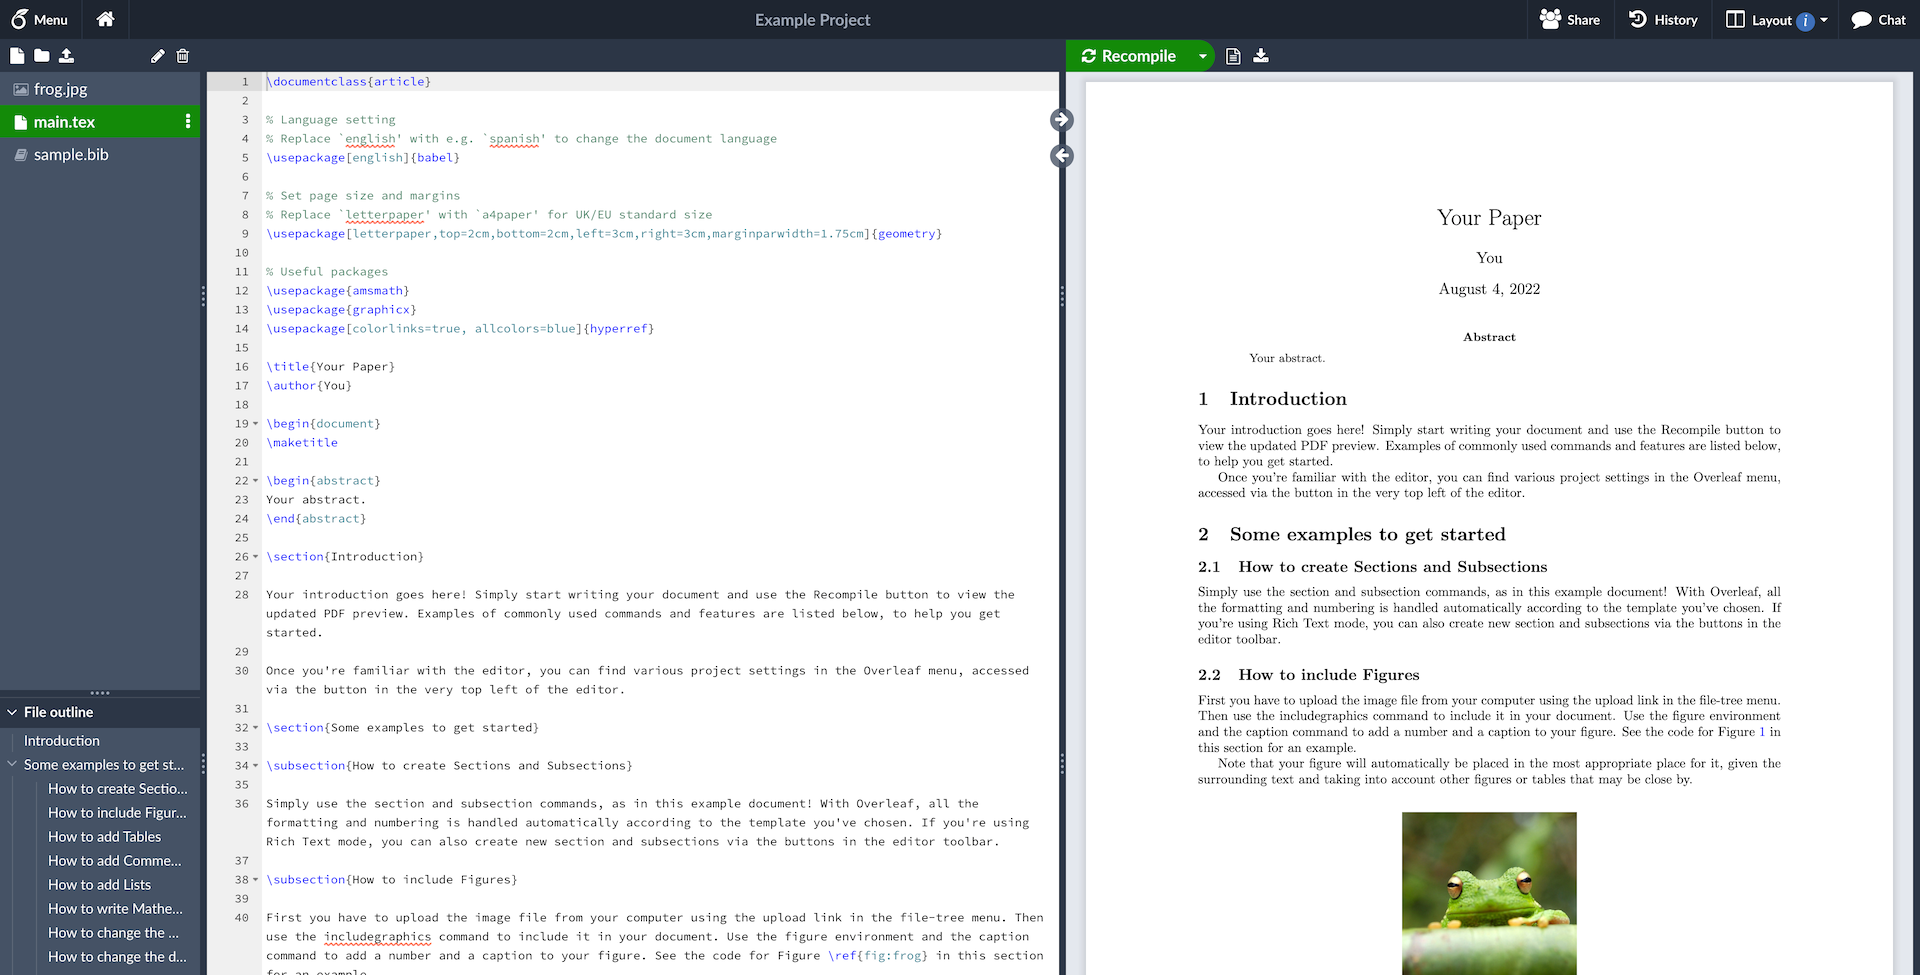
\includegraphics[width=0.85\textwidth]{img/overleaf.png}
  \caption{\centering{Overleaf editor. Source: \href{https://en.wikipedia.org/wiki/Overleaf}{wikipedia.org}}}
  \label{fig:overleaf_screenshot}
\end{figure}

\subsection{Versions}
\label{subsec:overleaf-versions}
Overleaf is available in three versions, which differ in features, levels of collaboration, deployment models, and costs.
Overleaf Community Edition (CE) is the free, self-hosted version designed for individual users and small teams. Overleaf Server Pro is the paid, self-hosted version tailored to organizations that offers advanced collaborative and administrative features. The cloud-based of Overleaf, instead, is offered as a service, comes in different tiers, and provides advanced features as well as various possibilities for integration.

\subsubsection{Overleaf Community Edition}
Overleaf CE\footnote{Overleaf Community Edition - \href{https://github.com/overleaf/overleaf/tree/main}{https://github.com/overleaf}} is free, open-source, and self-hosted. Although many collaborative features and integrations advertised by the company are not available in this version, it still represents an affordable solution for individual users and small research groups. Installation and setup are supported by the Overleaf Toolkit\footnote{Overleaf Toolkit - \href{https://github.com/overleaf/toolkit}{https://github.com/overleaf/toolkit}} and Docker, allowing users to deploy the software wherever they prefer. Beyond full control over data, privacy, and customization, this version has no restrictions on document compilation and supports unlimited collaborators per project. However, the company does not provide any support to the users, who have to rely on the community. 

\subsubsection{Overleaf Server Pro}
Overleaf Server Pro\footnote{Overleaf Server Pro - \href{https://www.overleaf.com/for/enterprises}{https://www.overleaf.com/for/enterprises}} is the self-hosted solution designed for organizations. It requires a paid license, which also guarantees priority support from the company. Compared to the CE, this version enables collaborative features, allows integration with Git, and provides a private template management system to share templates within the organization. Server Pro also supports SAML-based Single Sign On (SSO) and integrates some software optimizations.

\subsubsection{Overleaf}
Overleaf is the cloud-based solution for individual users, teams, and organizations. It is offered as a service and requires a paid subscription plan to access advanced features, but allows limited use with the free plan. Every paid plan enables all the collaboration features and allows integration with third-party services such as GitHub and Dropbox, as well as reference management software such as Mendeley and Zotero. In addition, they integrate Writefull, an AI-powered writing assistant, by default.
Groups and Commons tiers provide an advanced admin panel that, depending on the subscription, allows Single Sign On integration, automated user registration through LDAP or SAML, user account management and access to user metrics. Clearly, it doesn't require self-management of resources and guarantees automated updates and backups.
Since the free, standard, pro, and student plans are proposed for individuals, only Groups and Commons plans will be considered in this context and then unified as a unique solution.

\subsection{Hardware requirements and limitations}
Before diving into the sustainability assessment, it is necessary to clarify what specifications are required by self-hosted versions. Hardware requirements are published in the official GitHub wiki of Overleaf\footnote{Overleaf CE and Server Pro hardware requirements - \href{https://github.com/overleaf/overleaf/wiki/Hardware-Requirements}{https://github.com/overleaf}} and are shared between the two versions.
The minimal install requires 2 CPU cores and 3GB of RAM to support approximately 5 concurrent users. Then, it is suggested to add 1 CPU core and 1GB of memory for every 5/10 concurrent users. Therefore, the range provided by this rule is assumed to determine whether the allocation of resources is conservative (i.e. every 10 users) or aggressive (i.e. every 5 users). Allocating fewer or more resource could lead, respectively, to under-provisioning and over-provisioning.

With regard to storage allocation, Overleaf recommends using local disk storage for instances with fewer than 1000 users, which is approximately the limit suggested for the Community Edition. The maximum size allowed for a project is 500MB, but it is recommended not to exceed 100MB due to the size limit introduced by git integration. Considering that the size of the docker image is about 1GB and a full TeXLive installation is nearly 5GB, the storage requirement could be estimated as follows:
\[
\text{Storage}_{\text{exp}} = \text{Project size}_{\text{avg}} \times \text{Projects per user}_{\text{avg}} \times \text{Users}_{\text{exp}} \times \text{Backup space}
\]
For example, considering the base size, 25MB per project, 20 projects per user, and 300 users, while adding approximately 80\% of the space for backups, the required storage can be estimated at around 300GB.

The major constraint of Overleaf CE is that it supports only a single server deployment, meaning that all services, including the database, projects storage, and LaTeX compilation, must run on the same machine. This implies a severe limitation on scalability. In contrast, Overleaf Server Pro supports horizontal scaling, allowing multiple instances to share the workload through a load balancer and centralized storage. In this case, local storage is no longer supported and S3-compatible storage is recommended.

Table \ref{tab:overleaf_requirements} summarizes what has been discussed in this section, considering 300 expected users and 30 expected concurrent users.


\begin{table}[ht!]
    \centering
    % \small
    % \scriptsize
    % \tiny
    % \footnotesize
    \renewcommand{\arraystretch}{1.5} % Adjust row height
    \begin{tabular}{|>{\centering\arraybackslash}m{4cm}|>{\centering\arraybackslash}m{2.5cm}|>{\centering\arraybackslash}m{2.5cm}|>{\centering\arraybackslash}m{2.5cm}|>{\centering\arraybackslash}m{2.5cm}|}
        \hline
        \multirow{2}{*}{\textbf{Specification}} & \multicolumn{4}{c|}{\textbf{Overleaf provisioning - resource allocation}} \\
        \cline{2-5}
        & Under & Conservative & Aggressive & Over \\
        \hline
        Exp. number of Users & \multicolumn{4}{c|}{300}  \\
        \hline
        Exp. number of concurrent users & \multicolumn{4}{c|}{30} \\
        \hline
        Number of processors (or virtual processors) & 2 CPUs & 5 CPUs & 8 CPUs & 10 CPUs \\
        \hline
        Quantity of memory & 3 GB & 6 GB & 9GB & 12GB \\
        \hline
        Storage & \multicolumn{4}{c|}{300 GB} \\
        \hline
    \end{tabular}
    \caption{Overleaf hardware requirements for a large group of users}
    \label{tab:overleaf_requirements}
\end{table}

\section{Assessment of Overleaf through the sustainability framework}
\label{sec:4.2_overleaf_apply}
Universities aim to continuously improve academic productivity. In scientific departments and faculties, document production is often done with LaTeX, which offers better document control and scientific formatting compared to the traditional word processors. However, LaTeX comes with a steep learning curve, and its installation on user devices is not always fast and intuitive. Moreover, collaboration between users requires specific tools such as git or other version control systems, which require additional effort to become familiar with the workflow. In the context of digitization, this study assumes that the university would like to adopt a more efficient solution for the preparation of documents such as theses, articles, and publications by students, teachers, and researchers, particularly in scientific faculties.

Following the sustainability framework defined in the previous chapter, this section applies the methodology to Overleaf, evaluating its versions and whether they align with universities' needs and sustainability criteria. Each dimension is analyzed through its respective indicators. However, given the interconnections between certain indicators, some of them will be discussed together.
For each sustainability dimension, the results of the framework will be presented, providing an overview of Overleaf’s sustainability performance. A discussion and interpretation of the findings will be provided in the next chapter.

\bigskip

\subsection{Economic sustainability of Overleaf}
\label{subsec:overleaf-economic}
\medskip

\subsubsection{Return of expanses}
The return of expenses indicator analyzes the relationship between the cost of the DET and the value it generates. Overleaf has significant differences in costs among its versions, which are proportional to the number of features available. In the case of the Community Edition, the cost is determined by the amount of work required to install and configure the software, as well as the startup and maintenance of the hardware infrastructure. Apparently, this version could have a high initial return of expenses, which may decline as the number of users grows due to its limitations in scalability and administrative control. On the other hand, cloud-based and Server Pro versions are designed for enterprises and institutions, and the licensing (or subscription) costs are far from negligible. The generated value of these versions is nearly the same, with the self-hosted version potentially increasing cost efficiency as the number of users grows. However, the determining factor is the definition of generated revenue. For example, if the generated revenue is determined by rapid user adoption, the cloud-based may be preferred, while if the generated value is determined by control over the infrastructure, Server Pro may be preferred. Due to the difficulty of carrying out a systematic assessment, this indicator is not considered in the case study. 

\subsubsection{Provisioning and scaling policies}
The provisioning and scaling policies indicators evaluate, respectively, the cost of resources per user and the waste of resources. The technical characteristics of each version significantly impact resource management. Overleaf CE is limited to a single server machine, making scaling a critical factor and requiring accurate provisioning to avoid excessive costs. Server Pro instead supports horizontal scaling, enabling the distribution of computational load across multiple instances as needed. Meanwhile, the cloud-based version relies on a digital infrastructure shared among multiple users and organizations, ensuring optimal provisioning and efficient scaling. Clearly, the limited possibilities of the Community Edition are sufficient to assign a bad score, while the potential of Server Pro to reduce waste and increase cost efficiency in the long term justifies a good score. 

The assessment of this indicator is limited to a high-level perspective. A comprehensive study would require detailed knowledge of the infrastructure hosting Overleaf, as well as the associated and estimated costs of resource usage, which fall beyond the scope of this thesis.   

\subsubsection{Vendor lock-in and exit costs}
The vendor synergies and exit costs indicators evaluate the degree of dependency on the vendor’s ecosystem and the financial and technical effort required for migration. Regardless of the version, Overleaf is founded on standard LaTeX, which is an open-source technology. Therefore, it doesn't rely on proprietary formats or standards. Any project produced with Overleaf can be opened and modified with other LaTeX editors and can be compiled using other LaTeX distributions. In addition, users are allowed to export their projects at any time. In self-hosted versions, access to users projects is granted to the admins through their control dashboard, allowing mass export of projects inside the organization's workspace. 

Taking these factors into account, there is no evidence of vendor lock-in practices by the company in any version. However, some features may exercise a soft lock-in that does not affect the final outcome. For example, its ready-to-use nature and collaborative features may require users to make a considerable effort to gain expertise with local LaTeX distributions and familiarize themselves with alternative collaborative methods.

When migrating from Overleaf, the costs are determined only by the technical effort required for the digital infrastructure (if self-hosted) and for data export, which can be delegated to the individual users (except for the cloud version).

\bigskip

\subsection{Technical sustainability of Overleaf}
\label{subsec:overleaf-technical}
\medskip

\subsubsection{Availability and Reliability}
The availability and reliability indicators evaluate whether the software is operational and functions correctly. In the case of Overleaf, given its use for document production, its use is not confined to fixed times. Therefore, it must always be available. Furthermore, since it relies on the Internet connection, a high level of reliability is essential, particularly for content saving. However, compiler failures may rarely occur without significant consequences.

To assess the availability of Overleaf CE and the cloud-based version, both were monitored using Uptime Kuma\footnote{Uptime Kuma - \href{https://uptime.kuma.pet/}{https://uptime.kuma.pet}}, a popular self-hosted monitoring tool.
As shown in Figure \ref{fig:overleaf_availability}, the Community Edition instance maintained availability of nearly 100\% over a month. The cloud-based version showed the same result according to Uptime Kuma, which was also confirmed on the official status page\footnote{Overleaf Status Page - \href{https://status.overleaf.com/}{https://status.overleaf.com}}. 

\begin{figure}[ht!]
  \centering
  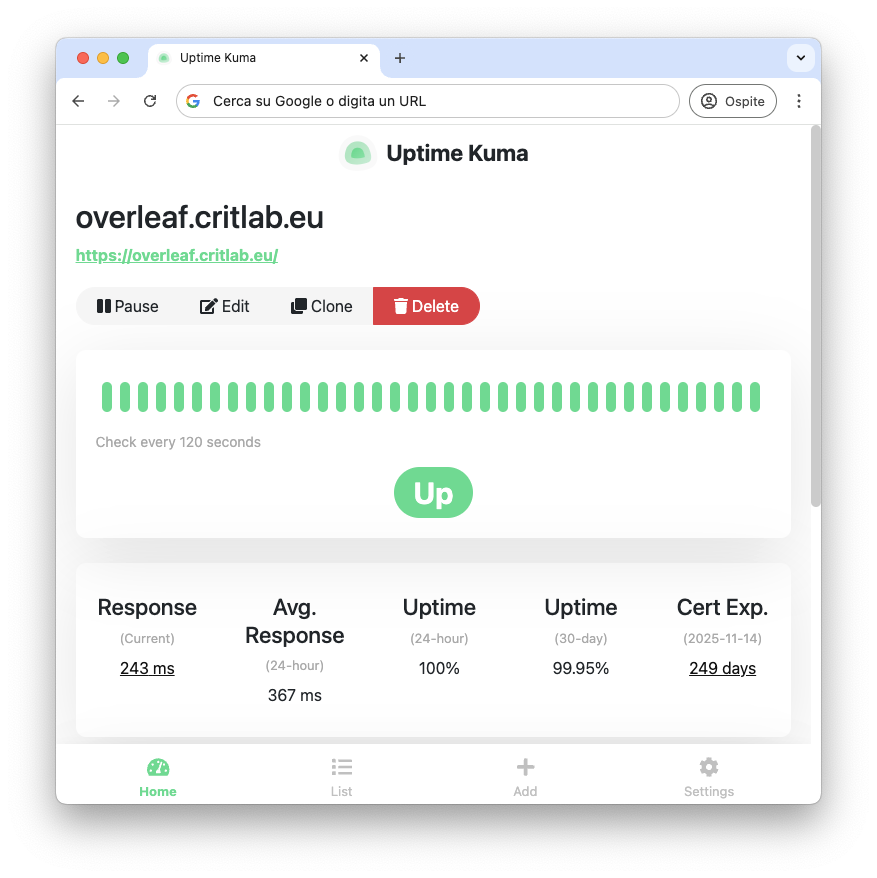
\includegraphics[width=0.6\textwidth]{img/overleaf_availability.png}
  \caption{\centering{Monitoring of Overleaf Community Edition with Uptime Kuma.}}
  \label{fig:overleaf_availability}
\end{figure}

To the best of the author's knowledge, Overleaf ensures reliability in all its versions, as confirmed for the cloud-based version by the incident history on its status page. 

\subsubsection{Scalability}
The scalability indicator assesses the ability of the system to meet changing demands. While for the cloud-based version this aspect is addressed by the service provider, the self-hosted versions support different levels of scalability that should be considered with respect to the underlying infrastructure. The Community Edition does not support any scalability techniques, thus the requirement is not satisfied. Instead, Server Pro supports load balancing and horizontal scaling, meeting the minimum requirement. Both versions support vertical scaling, but it will likely require manual intervention.

\subsubsection{Maintainability}
The maintainability indicator evaluates the ease of configuring, updating, and upgrading the software. As with the previous indicator, the cloud-based version is excluded, since the vendor is in charge of these operations. For Overleaf Community Edition and Server Pro, the level of maintainability is nearly the same, since they share tools and documentation. Before the introduction of Overleaf Toolkit, updates and upgrades were made through Docker images, and actually it is still possible to use this method. However, updates made by skipping some intermediate versions could lead to compatibility issues with dependencies. Now, these operations are performed through Overleaf Toolkit, which provides a useful script to simplify the process and limit the possibility of error.

The documentation is published in the official GitHub repository. It is not particularly complete, and sometimes appears hasty and informal, but it contains all the essential information. As for support, it is granted only to the Server Pro license owners, while for community edition users, support is delegated to the community.

Overall, the level of maintainability of both versions meets the minimum requirement, but the lack of direct support for the Community Edition should be considered. 

\subsubsection{Adaptability}
The adaptability indicator assesses whether the software supports integrations with university infrastructure and third-party services. Overleaf Community Edition does not support any built-in integrations with third-party tools. Overleaf Server Pro, however, supports Git integration and Single Sign-On, allowing user login to be integrated with the university administration system. In contrast, Overleaf Cloud provides several built-in integrations, such as Dropbox, GitHub, and reference management software. It also integrates generative AI for writing assistance.  

\subsubsection{Repairability}
The software repairability indicator evaluates whether the software and the underlying infrastructure allow interventions when issues and malfunctions occur. The key determining factors are the nature of the underlying infrastructure and whether the software is open-source or proprietary. Being open-source, Overleaf Community Edition, as well as Server Pro, allows interventions at both the code and infrastructure levels. If the software is not working properly, IT staff can take immediate action to resolve the issue and restore functionality. In contrast, the cloud-based version is fully managed by an external provider, preventing direct intervention and limiting the university's control in the event of malfunctions.

\bigskip

\subsection{Social sustainability of Overleaf}
\label{subsec:overleaf-social}
\medskip

\subsubsection{Community awareness}
The community awareness indicator assesses whether the service provider keeps the community up to date on changes and decisions that could affect the sustainability of the system. In this case, the indicator is applied uniformly across the three versions of Overleaf. The official Overleaf website has a blog section where the company publishes articles, news, and tutorials, but also changelogs, new feature announcements, and information about changes affecting the system. In addition to the infrequent publication of such information, it is evident that these updates are not driven by sustainability purposes, as this term is rarely or not mentioned at all.

\subsubsection{Involvement in sustainability}
The involvement in sustainability indicator measures the distance between the company and a sustainability claim. This indicator is evaluated by exploring the official website and searching for sustainability claims on the Web. The research was conducted by searching for related keywords such as "sustainability" and "environmental" along with other similar terms, in combination with "Overleaf" or organizations associated with it, as identified on the Overleaf website. Even though a more exhaustive investigation is necessary, this search did not produce any positive results. As a result, the company distance is more than one "hop".

\subsubsection{Inclusion}
The inclusion indicator states whether the software is compliant with accessibility standards. The evaluation was first conducted by searching for related keywords such as "accessibility" and "inclusion" in combination with "Overleaf" to find accessibility reports on the software. Then, compliance with WCAG was assessed using WAVE Evaluation Tool. Finally, although it is not aligned with WCAG, Google's Lighthouse tool in Google Chrome was used to confirm the findings of WAVE. Both tools were run in the editor view, with an empty project.

The results of the research show that no accessibility report is readily available. The evaluation with WAVE highlights the presence of many contrast errors and some missing alternative text for images, while other requirements, such as ARIA labels and structural elements, are fully compliant. Lighthouse, instead, identified some errors that did not align with WAVE's results. However, the tool provided three different scores for the same view, ranging from 65 to 85, and therefore its results are excluded from the evaluation.

Given the complexity of the software, it can be considered compliant with the minimum accessibility requirements.

\subsubsection{Privacy Policy}
The privacy policy indicator evaluates how users' data is collected and used. The assessment was first conducted by studying the privacy policy available on the official website, then identifying any sub-processors, and finally verifying the readability of the policy. 

Overleaf stipulates confidentiality contracts with third-party services and claims that user data may be shared with such services. However, many sub-processors are not explicitly mentioned in the privacy policy. Instead, they are listed on a separate page, which appears to be difficult to access within the website. Overleaf has numerous sub-processors, such as Google, Amazon, Heroku, Paypal, OpenAI, and many others (for the complete list, refer to Appendix \ref{cha:attachment_overleaf_comparison}).  Furthermore, information about the use of collected data by the integrated AI assistants, such as Writefull and TeXGPT, is displayed only while using the editor. Overleaf also uses analytics tools, such as Google Analytics.

The readability test was conducted using Readable\footnote{Readable - \href{https://readable.com/}{https://readable.com}}, Hemingway Editor\footnote{Hemingway Editor - \href{https://hemingwayapp.com/}{https://hemingwayapp.com}}, and GoodCalculators\footnote{GoodCalculators - \href{https://goodcalculators.com/}{https://goodcalculators.com}}, leading to the following results:
\begin{itemize}[noitemsep, topsep=4pt, parsep=0pt, partopsep=0pt]
    \item Flesch-Kincaid Grade Level: 12.7 (Readable), 13 (Hemingway Editor and GoodCalculators)
    \item Flesch Reading Ease: 39.7 (Readable), 35.4 (GoodCalculators)
    \item Gunning Fog Index: 14.6 (Hemingway Editor)
\end{itemize}
To obtain a good score, the Flesch-Kincaid Grade Level and Gunning Fog Index should be lower than 10, while Flesch reading ease score should be greater than 60. Thus, the cloud-based version does not satisfy the requirements of ethical approach and good readability, but it is compliant with the GDPR. 

The self-hosted versions, instead, are regulated by the university's own policy, since it is the only data processor. Clearly, if the university decides to integrate external analytics tools or to deploy the services to an external cloud infrastructure, then sub-processor are involved. Due to the total freedom in managing data processing, the self-hosted versions largely meet the requirements. 

\subsubsection{Capacity}
The capacity indicator evaluates whether the software is likely to generate internal capacity. The result is immediate because the cloud version is completely outsourced, while the self-hosted versions require skills and knowledge of deployment models, scaling techniques, and many other technical concepts. Given the higher complexity of Overleaf Server Pro compared to the Community Edition, the former requires more expertise than the latter. By the way, a significant factor to consider is that the self-hosted version is open-source and may encourage to contribute to the project. 

\bigskip

\subsection{Pedagogical sustainability of Overleaf}
\label{subsec:overleaf-pedagogical}
\medskip

\subsubsection{Engaged with instructional practices}
This indicator highlights whether the DET is founded on solid instructional practices or is actively involved in pedagogical research. As with previous indicators, the evaluation was first conducted by searching for related keywords, such as "pedagogical", "teaching", and "education" in combination with "Overleaf", to find evidence of the use of instructional practices or active research. Even if the research did not produce positive results, it was found that Overleaf is proposed as a digital education technology. The focus, aside from research, is on teaching, since the company claims that its features, such as documentation and presentation production, as well as template sharing, can improve the teaching experience. Anyway, these features were not specifically designed for teaching, but to increase writing productivity, especially for researchers.

\subsubsection{Usability}
The usability indicator verifies how efficient and user-friendly a digital technology is. The evaluation was conducted by reviewing the criteria described in Section \ref{sec:3.1_framework_structure}. Since Overleaf is focused on LaTeX, which has a significant learning curve, an important aspect is how the editor simplifies its use. A summary of the factors considered is presented in the following list:
\begin{itemize}[noitemsep, topsep=4pt, parsep=0pt, partopsep=0pt]
    \item Learnability - Overleaf provides a comprehensive and free-to-access LaTeX documentation, as well as tutorials for Overleaf and crash courses. Basic tasks such as simple text formatting (e.g., italic, bold, lists) and insertion of hyperlinks, tables, and formulas can be done with the toolbar, allowing users to familiarize themselves with the editor.
    \item Efficiency of use - Overleaf provides a comprehensive list of hotkeys for common tasks. In addition, it also provides auto-complete features for commands, images, references, and many other elements. The editor offers a split-screen view with the project navigator and the output file preview on the sides.
    \item Error prevention and user control - Overleaf identifies some errors (e.g. unclosed commands) before compilation. Otherwise the compiler will list the errors, which unfortunately are often not self explaining. The toolbar and the hotkeys help to prevent writing errors.
    \item Feedback and transparency - Typically, when the software faces an issue, such as connection errors or rendering errors, it displays a message to the users. However, sometimes it does not provide any feedback, making it difficult to understand the state of the system (e.g., it is assumed that the software is connected because there are no error messages).   
    \item Integrations and customization - Integrations are available only in paid versions, and the cloud version supports more integrations than Overleaf Server Pro. Overleaf allows basic customization such as font family, font size, line height, and editor theme. Other customizations relate to auto-completion and compiler configuration.
\end{itemize}
Considering that environmental setup is no longer necessary, Overleaf meets the requirements, but a more detailed assessment would be necessary. 

\subsubsection{Purpose and Impact on education}
The purpose and impact on education indicators cannot be evaluated in a purely systematic way, but should be discussed to obtain a better picture of the problem. Purpose refers to the motivations that lead to the adoption of a technology, while impact on education tries to understand what are the implications of this adoption.

In this study, it is assumed that the university wants to adopt Overleaf to improve document preparation for students, teachers, and researchers. In scientific faculties, LaTeX is widely used for many purposes, and the introduction of Overleaf in the existing workflow would bring several benefits, such as greater collaboration, less complexity in setup and configuration, and many others. For example, a student who is preparing his final dissertation can easily share the project with its supervisor, who can check the content and suggest changes through the review feature. If the previous workflow is based on local LaTeX, these operations were probably done via e-mail, and this clearly represents an improvement. Another example: a group of researchers that is preparing an article can easily share the project among the team members, ensuring that they work always on the latest version. These use cases validate both the purpose and the impact on education.

But what if the university wanted to adopt Overleaf for word processing? Clearly, this scenario is the completely opposite of the previous one, adding unnecessary complexity, requiring additional effort, and probably disrupting the existing workflow. The steep learning curve and required skills would lead to a negative impact on education. Overleaf is not suitable for everyone; it has a strong orientation toward STEM disciplines, and this must be carefully considered when evaluating its adoption.

To conclude, based on the assumption, Overleaf can improve document preparation within the institution, and its impact on education is positive.

\bigskip

\subsection{Environmental sustainability of Overleaf}
\label{subsec:overleaf-environmental}
\medskip

\subsubsection{Energy and raw material consumption, carbon emissions}
These indicators estimate the environmental impact of the technology under examination. To find an environmental assessment about Overleaf, a search was conducted using related keywords such as "environmental", "assessment", "emissions", and "energy" in combination with "Overleaf". Unfortunately, the research did not produce any result, but some considerations can be inferred by looking at Overleaf's sub-processors.

Overleaf declares that it relies on Amazon AWS, Google Cloud Platform, Heroku and MongoDB Atlas for hosting. As discussed in Chapter \ref{cha:2_dets-and-sustainability}, the relationship between Big Tech companies and the environmental impact is far from trivial. Large data centers continue to rely on energy produced from fossil fuels due to their low cost and widespread availability. To meet renewable energy requirements, companies often rely on renewable energy certificates (RECs) \cite{khosravi_review_2024}\cite{stacey_pollution_2025}. Through RECs, companies claim to produce, elsewhere or in-site, an equivalent amount of renewable energy compared to the energy used by the data centers. However, this practice does not ensure that the data centers are actrually supplied by renewable energy, and RECs have been criticized for allowing companies to claim zero-emissions or low-impact status without substantial proof. Considering their low willingness to share data on environmental impact, the lack of transparency, and contribution to e-waste generation, software relying on big cloud providers cannot get a good score with these indicators.

For on-premises solutions, instead, the indicators are not applicable due to the lack of knowledge about the system that will host the software. Nonetheless, a neutral score is assigned because of the potential to rely on environmentally responsible infrastructures. 

\subsubsection{Sustainability in design and through design}
The sustainability in design indicator states how sustainability is considered as a software quality, while the sustainability through design indicator evaluates the impact the technology has on users. As shown in the assessment of community awareness indicator, there is no evidence that sustainability concerns were accounted for in the design phase. Moreover, some considerations can be done simply by using the software. First, the editor pushes users to compile frequently due to its association with the typical saving mechanism, which increases the computational load and related energy consumption. Then, the real-time collaboration feature requires a persistent connection to synchronize data. Finally, it is not clear whether the company uses a less efficient algorithm or fewer computational resources for free or cheaper plans. Deploying a self-hosted version to a sustainable infrastructure can mitigate these issues, but cannot solve them.

Regarding sustainability through design, the outcome is nearly the same. For example, the user interface does not show the user any information about resource usage. As another example, the software does not support any low-power or energy saving mode and users are not able to customize the software to significantly reduce its resource usage. To the best of the author's knowledge, Overleaf does not encourage sustainable practices through its software.

\section{Result}
\label{sec:4.3_overleaf_result}
The overall result of the assessment is shown in Figure \ref{fig:overleaf_result_overview}. Every row represents one of the 25 indicators within its dimension, while each column represents a version of Overleaf. As described in chapter \ref{cha:3_framework}, each color is associated with a score, where green is 1, yellow is 0, red is -1, and gray means not applicable. The final score is displayed at the bottom and is shown in relation to the number of indicators applied. 

\begin{figure}[ht!]
    \centering
    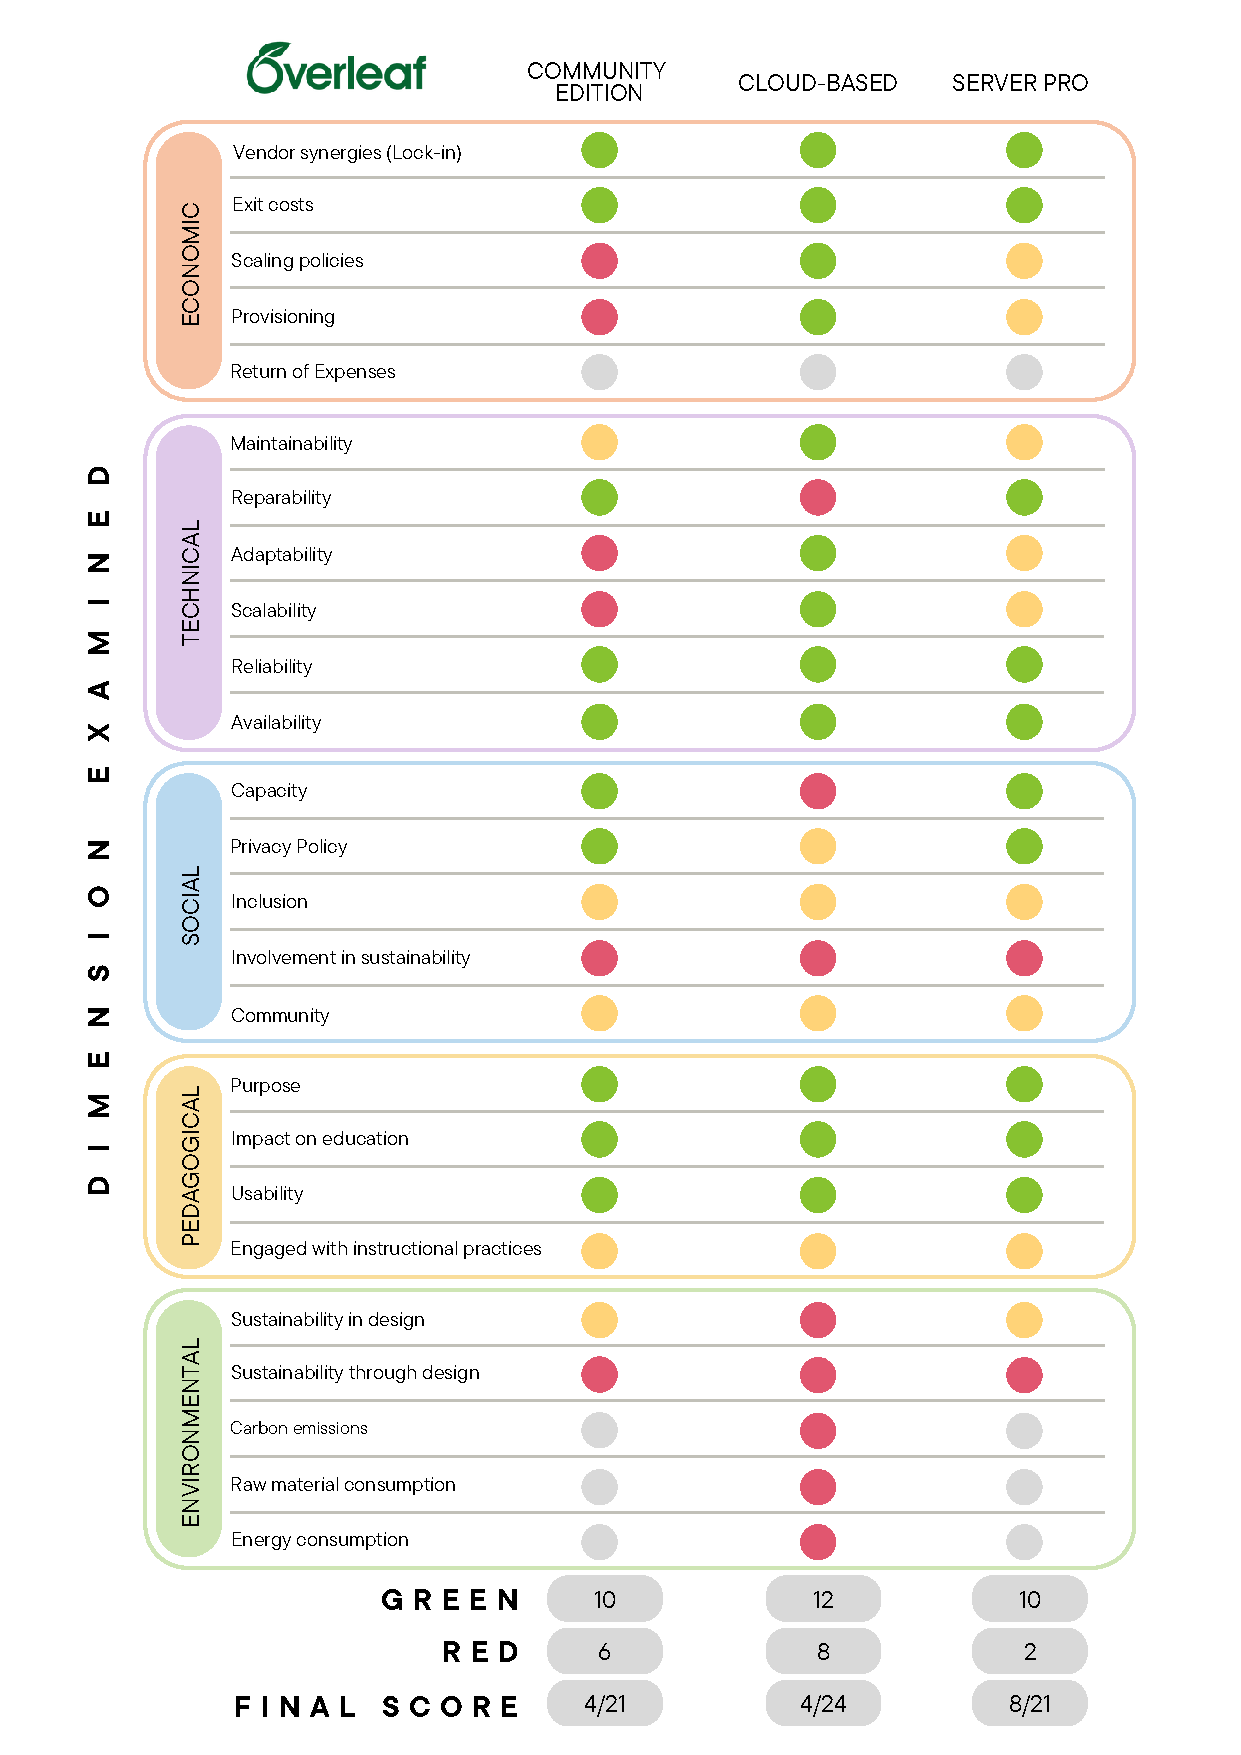
\includegraphics[width=1\textwidth]{attachments/overleaf_result_overview.pdf}
    \caption{Overall result of Overleaf's assessment}
    \label{fig:overleaf_result_overview}
\end{figure}

% ATTENZIONE aggiungere score verde e score rosso allo schema
% trattare l'argomento nelle conclusioni
% magari insieme alla parte sulle zone rosse

% PER PRESENTAZIONE: qual è il messaggio principale????